\documentclass[a4paper,11pt]{ltjsarticle}
\usepackage{base}
\title{}
\author{}
\date{}
\begin{document}
\begin{que}
\ce{Ag+},\ce{K+},\ce{PB^2+},\ce{Ca^2+},\ce{Zn^2+},\ce{CU^2+},\ce{Al^3+}のイオンを同じ濃度で含む水溶液がある.図は,各イオンを分離する操作である.(a)〜(i)の,金属を含む沈殿またはイオンの化学式を記せ.
\begin{figure}[H]
\centering
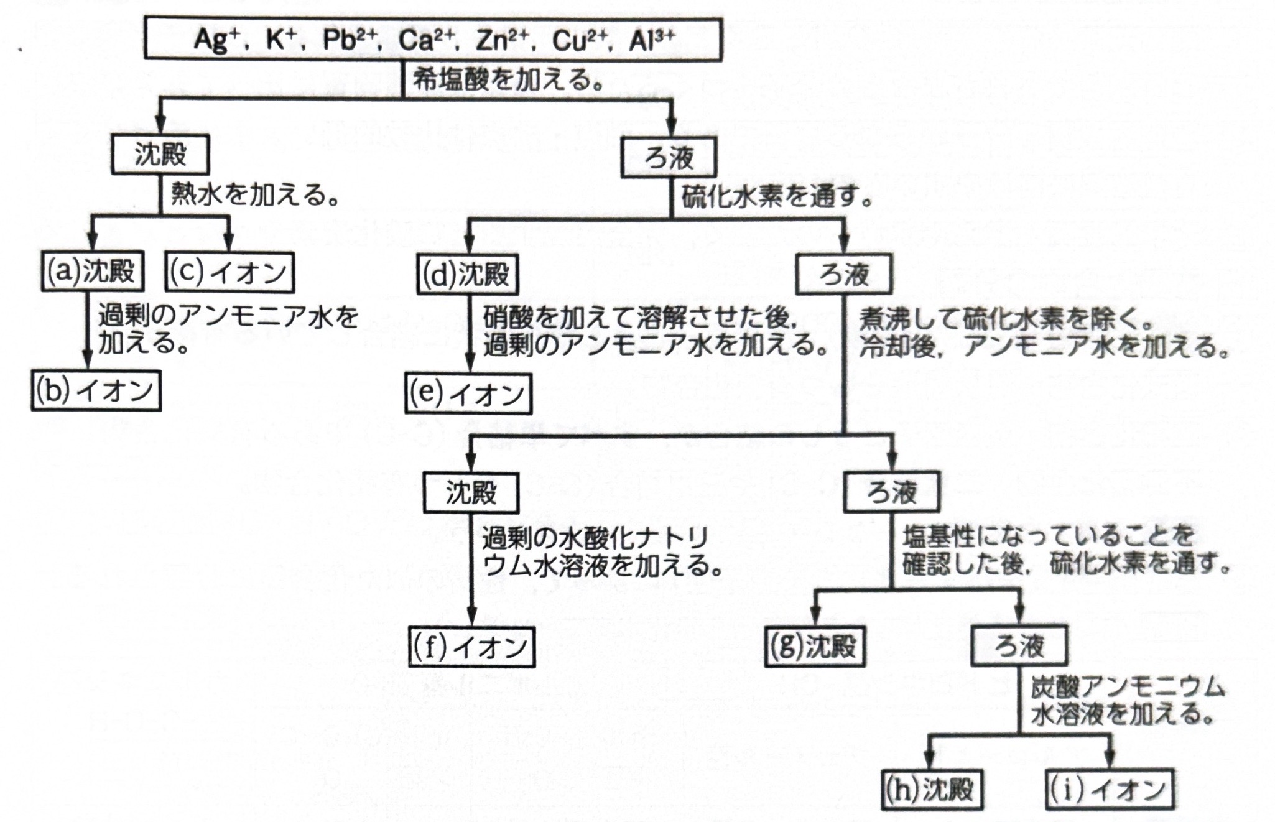
\includegraphics[width=13cm]{269.pdf}
\end{figure}
\end{que}
\newpage
\begin{que}
元素の質量百分率が炭素54.5$\%$,水素9.1$\%$で,分子量が88.0のエステルAがある.Aを加水分解するとカルボン酸とアルコールが生じた.
\begin{itemize}
    \item[(1)]Aの分子式を求めよ.
    \item [(2)]加水分解により生じたカルボン酸が銀鏡反応を示した.このとき考えられるAの構造異性体は何種類か.
    \item [(3)]加水分解に生じたアルコールを酸化したところ,その生成物は銀鏡反応を示した.Aの構造式を描け.
\end{itemize}
\end{que}
\newpage
  \begin{que}
    ベンゼン1molと塩素1molを反応させ,ベンゼンの水素1つを塩素で置換したい.
    \begin{itemize}
        \item [(1)]この反応を進行させるために必要な触媒を2通りあげよ.
        \item [(2)]この反応を何というか.
        \item [(3)]生成したベンゼン一置換体の名称を答えよ.
        \item [(4)]追加で1molの塩素を反応させたとき,考えられる生成物の構造式と名称を答えよ.
  \end{itemize}
    \end{que}
  \newpage
  \begin{que}
   次の分子式で表される芳香族化合物の異性体をすべて記せ.
   \begin{itemize}
    \item [(1)]\ce{C6H3Cl3}
    \item [(2)]\ce{C7H7Cl}
    \item [(3)]\ce{C9H12}
   \end{itemize}
  \end{que}
  \newpage
  \begin{que}  フェノールはベンゼン環に\fbox{あ}基がついた\fbox{い}酸で,水酸化ナトリウム水溶液に溶けて\fbox{う}となる.この水溶液に二酸化炭素を吹き込むと,炭酸はフェノールよりも\fbox{え}い酸なので,\fbox{お}反応によりフェノールが得られる.\\
  ベンゼン環に直接結合したヒドロキシ基は\fbox{か}と呼ばれ,アルコールとは異なる性質を示す.これを検出するには,\fbox{き}水溶液に加えて色が\fbox{く}〜\fbox{け}に変化することを確認すればよい.\\
  フェノールの代表的な製法である\fbox{こ}法では,プロピレンへのベンゼンの付加反応により生じる\fbox{さ}を酸化して得られる\fbox{し}を硫酸で分解してフェノールを得る.このとき,副産物として\fbox{す}も得られる.\\
  また,ベンゼンと濃硫酸を加熱することで得られる\fbox{せ}を中和した後,水酸化ナトリウムと融解することで\fbox{そ}が生じる.これを酸性にすることで,\fbox{た}反応によりフェノールが得られる.\\
 フェノールはベンゼンと比べて\fbox{ち}反応を受けやすい.例えば,フェノールに十分量の臭素水を加えると\fbox{つ}の白色沈殿が生じる.
 \begin{itemize}
    \item [(1)]文中に当てはまる語句などを答えよ.
    \item [(2)]\fbox{し}と\fbox{つ}の構造式を記せ.
 \end{itemize}
\end{que}
\newpage

\begin{que}
次の文中の化合物A〜Gの構造式を記せ.\\[8pt]
分子式\ce{C4H10O}の異性体の1つであるAを酸化すると,Bが得られた.Bは銀鏡反応ウィ示した.濃硫酸にAを加えて加熱すると,Cが得られた.Cに臭素を付加すると,不斉炭素原子を含まないDが得られた.Cに酸触媒を用いて水素を付加すると,Aとは異なるEが得られた.一方,Cの異性体の1つであるFに臭素を付加すると,不斉炭素原子を1個もつGが得られた.
\end{que}
\newpage
\begin{que}
    次の文中のA〜Cの構造式を記せ.\\[8pt]
エステルA~2.60gを加水分解すると,直鎖状のモノカルボン酸B~1.76gと1価アルコールC~1.20gが得られた.アルコールCを穏やかに酸化したときの生成物はフェーリング液を還元せず,また,ヨードホルム反応を示した.
\end{que}
\newpage
\begin{que}
次の文中の化合物A〜Cの構造式を記せ.\\[8pt]
分子式\ce{C5H12O}で表されるアルコールにはいくつかの構造異性体がある.不斉炭素原子を持たないアルコールAを濃硫酸の存在下で加熱すると,互いにシス-トランス異性体でない,分子式\ce{C5H10}の化合物BとCが生成した.また,BとCに適当なさんを触媒として水を付加させると,どちらもAが主に生成した.
\end{que}
\newpage
\begin{que}
炭素,水素,酸素からなるヒドロキシ酸Aについて,次のことがわかっている.\begin{itemize}
    \item A~15.0mgを完全燃焼させると,二酸化炭素17.6mg,水5.4mgが得られた.
    \item Aの分子量は150であった.
    \item A~75mgと十分量のメタノールとの混合物に濃硫酸を加えて温めると,89mgのエステルBが生成した.ただし,反応は完全に進行したものとする.
    \item B~89mgに十分量の無水酢酸を加えて温めたところ,エステルC 131mgが得られた.ただし,反応は完全に進行したものとする.
    \item Aは不斉炭素原子を持つ.
\end{itemize}
このとき,次の問いに答えよ.
\begin{itemize}
    \item [(1)]Aの分子式を求めよ.
    \item [(2)]Aにはカルボキシ基,ヒドロキシ基がそれぞれいくつあるか.
    \item [(3)]Aの構造式を記せ.ただし,不斉炭素原子は\ce{C^*}と表記せよ.
\end{itemize}
\end{que}

\end{document}